\section{1174009 - Dwi Yulianingsih}
\subsection{Teori}
\begin{enumerate}

	\item Jelaskan apa itu binary classification dilengkapi ilustrasi gambar sendiri.
	\hfill\break
	Binary classification adalah konsep dasar yang melibatkan klasifikasi data menjadi dua kelompok. Baca terus untuk beberapa wawasan dan pendekatan tambahan. Binary classification atau klasifikasi biner melibatkan pengelompokan data ke dalam dua kelompok, mis. apakah pelanggan membeli produk tertentu atau tidak (Ya / Tidak), berdasarkan variabel independen seperti jenis kelamin, usia, lokasi, dll.

	\begin{figure}[H]
	\centering
		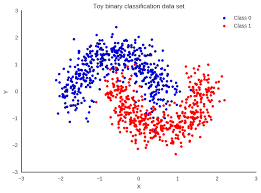
\includegraphics[width=4cm]{figures/1174009/tugas2/materi/1.png}
		\caption{Binary classification.}
	\end{figure}

	\item Jelaskan apa itu supervised learning dan unsupervised learning dan clustering dengan ilustrasi gambar sendiri.
	\hfill\break

	\begin{itemize}
		\item Supervised Learning
		\hfill\break
		Sebuah algoritma pembelajaran mesin yang dapat menerapkan informasi yang sudah ada dalam data dengan memberikan label tertentu, misalnya data yang telah diklasifikasikan sebelumnya (diarahkan). Algoritma ini mampu memberikan target untuk output yang dilakukan dengan membandingkan pengalaman belajar masa yang sudah lampau. Supervised Learning adalah tugas pembelajaran untuk memetakan fungsi yang memetakan input ke output melalui contoh pasangan input-output. Ini terdiri dari data pelatihan berlabel yang terdiri dari kombinasi contoh pelatihan. Dalam pembelajaran yang diawasi, setiap contoh adalah pasangan yang terdiri dari objek input (biasanya vektor) dan nilai output yang diinginkan (juga disebut sinyal pengawas). Algoritma pembelajaran yang mulai menganalisis data pelatihan dan menghasilkan fungsi yang disimpulkan, yang dapat digunakan untuk memetakan contoh baru. Skenario optimal akan memungkinkan algoritma menentukan label kelas dengan benar untuk instance yang tidak terlihat. Ini membutuhkan algoritma pembelajaran untuk menggeneralisasi data pelatihan untuk pembelajaran yang tidak terlihat dengan cara yang "masuk akal" (lihat bias induktif). Tugas paralel dalam psikologi manusia dan hewan sering disebut sebagai konsep pembelajaran.

		\begin{figure}[H]
		\centering
			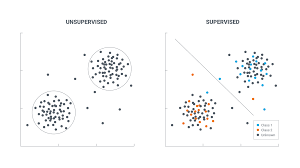
\includegraphics[width=4cm]{figures/1174009/tugas2/materi/2.png}
			\caption{Supervised Learning.}
		\end{figure}

		\item Unsupervised Learning 
		\hfill\break
		Berbeda dengan Supervised Learning, Unsupervised Learning ialah sebuah pembelajaran mesin tanpa pengawasan adalah pembelajaran mesin yang digunakan pada data yang tidak memiliki informasi yang dapat diterapkan secara langsung (tidak diarahkan). Algoritma ini diharapkan dapat menemukan struktur tersembunyi dalam data yang tidak berlabel. 

		\begin{figure}[H]
		\centering
			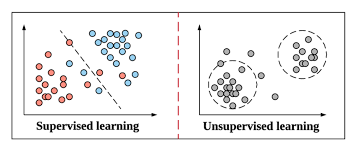
\includegraphics[width=4cm]{figures/1174009/tugas2/materi/3.png}
			\caption{Unsupervised Learning.}
		\end{figure}

		\item Clustering
		\hfill\break
		Clustering adalah tugas pengelompokan kelompok objek yang tampaknya menjadi objek dalam kelompok yang sama (disebut cluster) lebih mirip (dalam beberapa kasus) satu sama lain daripada kelompok lain (cluster). Ini adalah tugas utama penambangan data eksplorasi, dan teknik umum untuk analisis data statistik, yang digunakan di banyak bidang, termasuk pembelajaran mesin, pengenalan pola, analisis gambar, pencarian informasi, bioinformatika, kompresi data, dan grafik komputer. Analisis Cluster sendiri bukan merupakan salah satu algoritma spesifik, tetapi tugas umum yang harus diselesaikan. Ini dapat disepakati dengan berbagai algoritma yang berbeda secara signifikan dalam memahami mereka tentang apa itu cluster dan bagaimana memfasilitasinya secara efisien. Gagasan populer tentang cluster termasuk kelompok dengan jarak kecil antara anggota cluster, area padat ruang data, interval atau distribusi statistik tertentu. 

		\begin{figure}[H]
		\centering
			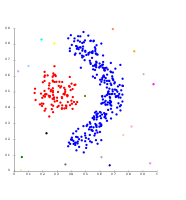
\includegraphics[width=4cm]{figures/1174009/tugas2/materi/4.png}
			\caption{Clustering.}
		\end{figure}
	\end{itemize}
	
	\item Jelaskan apa itu evaluasi dan akurasi dari buku dan disertai ilustrasi contoh dengan gambar sendiri.
	\hfill\break
	Evaluasi dan Akurasi adalah tentang bagaimana kita dapat meningkatkan model yang bekerja dengan mengukur akurasinya. Dan beberapa akan disetujui sebagai benar. Kita dapat menganalisis kesalahan yang dibuat oleh model menggunakan matriks. Matriks ini memperdebatkan perdebatan tentang model, tetapi matriks ini bisa sedikit sulit untuk dipecahkan dengan kompilasi mereka yang sangat besar.

	\begin{figure}[H]
	\centering
		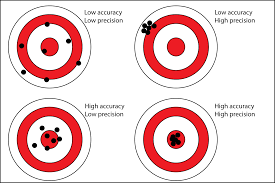
\includegraphics[width=4cm]{figures/1174009/tugas2/materi/5.png}
		\caption{Evaluasi dan Akurasi.}
	\end{figure}

	\item Jelaskan bagaimana cara membuat dan membaca confusion matrix, buat confusion matrix buatan sendiri.
	\hfill\break
	\begin{enumerate}
	\item Cara membuat dan membaca confusion matrix :
	\begin{itemize}
	\item Tentukan pokok permasalahan dan atributanya, misal gaji dan listrik.
	\item Buat pohon keputusan
	\item Lalu data testingnya
	\item Lalu mencari nilai a, b, c, dan d. Semisal a = 5, b = 1, c = 1, dan d = 3.
	\item Selanjutnya mencari nilai recall, precision, accuracy, serta dan error rate.
	\end{itemize}
	\item Berikut adalah contoh dari confusion matrix :
	\begin{itemize}
	\item Recall =3/(3+3) = 0,5
	\item Precision = 3/(3+5) = 0,375
	\item Accuracy =(3+5)/(3+5+5+3) = 0,5
	\end{itemize}
	\end{enumerate}

	\begin{figure}[H]
	\centering
		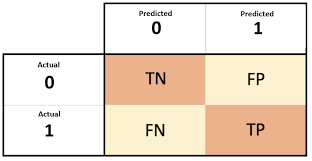
\includegraphics[width=4cm]{figures/1174009/tugas2/materi/6.png}
		\caption{Confusion Matrix.}
	\end{figure}

	\item Jelaskan bagaimana K-fold cross validation bekerja dengan gambar ilustrasi contoh buatan sendiri.
	\hfill\break
	\begin{itemize}
	\item Total instance dibagi menjadi N bagian.
	\item Fold yang pertama adalah bagian pertama menjadi data uji (testing data) dan sisanya menjadi training data.
	\item Lalu hitung akurasi berdasarkan porsi data tersebut dengan menggunakan persamaan.
	\item Fold yang ke dua adalah bagian ke dua menjadi data uji (testing data) dan sisanya training data. 
	\item Kemudian hitung akurasi berdasarkan porsi data tersebut.
	\item Dan seterusnya hingga habis mencapai fold ke-K.
	\item Terakhir hitung rata-rata akurasi K buah.
	\end{itemize}

	\begin{figure}[H]
	\centering
		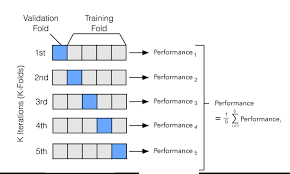
\includegraphics[width=4cm]{figures/1174009/tugas2/materi/7.png}
		\caption{K-fold Cross Validation.}
	\end{figure}

	\item Jelaskan apa itu decision tree dengan gambar ilustrasi contoh buatan sendiri.
	\hfill\break
	Decision tree atau pohon Keputusan adalah metode pembelajaran yang diawasi non-parametrik yang digunakan untuk klasifikasi dan regresi. Tujuannya adalah untuk membuat model yang memprediksi nilai variabel dengan aturan keputusan yang menentukan data fitur. Misalnya, dalam contoh di bawah ini, pohon keputusan belajar dari data untuk memperkirakan kurva dengan keputusan if-then-other lainnya. Semakin dalam pohon, semakin rumit aturan dan modelnya.

	\begin{figure}[H]
	\centering
		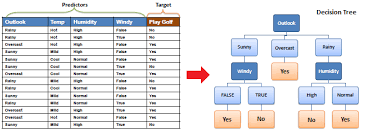
\includegraphics[width=4cm]{figures/1174009/tugas2/materi/8.png}
		\caption{Decision Tree.}
	\end{figure}

	\item Jelaskan apa itu information gain dan entropi dengan gambar ilustrasi buatan sendiri.
	\hfill\break
	\begin{enumerate}
	\item Information gain didasarkan pada data yang diperoleh pada saat penurunan setelah dataset dibagi berdasarkan atribut. Membangun pohon keputusan adalah semua tentang menemukan atribut yang memperoleh informasi tertinggi (misalnya, cabang yang paling homogen).
	\begin{figure}[H]
	\centering
		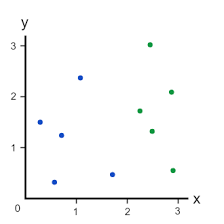
\includegraphics[width=4cm]{figures/1174009/tugas2/materi/9.png}
		\caption{Information Gain.}
	\end{figure}
	\item Entropi adalah ukuran yang dibaca dalam informasi yang sedang diproses. Semakin tinggi entropi, semakin sulit untuk menarik kesimpulan dari informasi itu. Membalik koin adalah contoh tindakan yang memberikan informasi acak. Untuk koin yang tidak memiliki afinitas terhadap kepala atau ekor, hasil lemparannya sulit diprediksi. Mengapa Karena tidak ada hubungan antara yang menentang dan hasil. Inilah inti dari entropi.
	\begin{figure}[H]
	\centering
		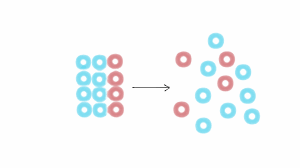
\includegraphics[width=4cm]{figures/1174009/tugas2/materi/10.png}
		\caption{Entropi.}
	\end{figure}
	\end{enumerate}

\end{enumerate}


\subsection{Praktek}
\begin{enumerate}
	\item Soal 1
	\hfill\break
	\lstinputlisting[firstline=10, lastline=13]{src/1174009/tugas2.py}
	Kode di atas digunakan untuk mengimpor atau mengirim library pandas sebagai pd. Kemudian ditentukan variabel "medan" untuk dipanggil dataset diperoleh dari data student-mat.csv. Hasilnya adalah sebagai berikut :
	\begin{figure}[H]
	\centering
		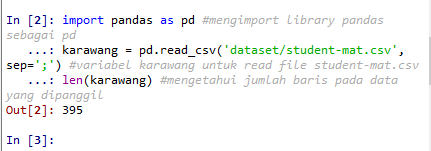
\includegraphics[width=4cm]{figures/1174009/tugas2/materi/hasil1.PNG}
		\caption{Hasil Soal 1.}
	\end{figure}

	\item Soal 2
	\hfill\break
	\lstinputlisting[firstline=18, lastline=21]{src/1174009/tugas2.py}
	Kode di atas ada bagian mendeklarasikan pass/fail nya data berdasarkan G1+G2+G3. Dengan ketentuan nilai pass nya yaitu sama dengan 30. kemudian pada variabel medan dideklarasikan jika baris dengan G1+G2+G3 ditambahkan, dan hasilnya sama dengan 35 maka axisnya 1. Hasilnya adalah sebagai berikut :
	\begin{figure}[H]
	\centering
		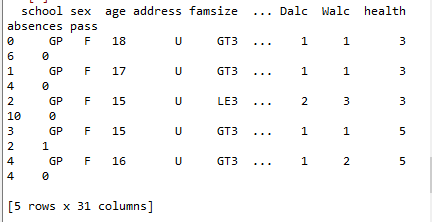
\includegraphics[width=4cm]{figures/1174009/tugas2/materi/hasil2.PNG}
		\caption{Hasil Soal 2.}
	\end{figure}
	
	\item Soal 3
	\hfill\break
	\lstinputlisting[firstline=26, lastline=30]{src/1174009/tugas2.py}
	One-hot encoding adalah proses di mana variabel kategorikal dikonversi menjadi bentuk yang dapat disediakan untuk algoritma ML untuk melakukan pekerjaan yang lebih baik dalam prediksi. Metode head ini digunakan untuk mengembalikan baris n atas 5 secara default dari frame atau seri data Karena saya memuat data menggunakan. Hasilnya adalah sebagai berikut :
	\begin{figure}[H]
	\centering
		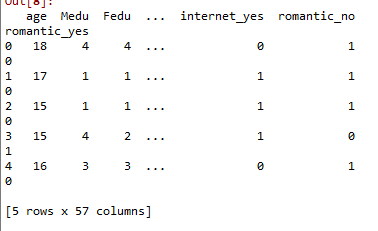
\includegraphics[width=4cm]{figures/1174009/tugas2/materi/hasil3.PNG}
		\caption{Hasil Soal 3.}
	\end{figure}

	\item Soal 4
	\hfill\break
	\lstinputlisting[firstline=35, lastline=52]{src/1174009/tugas2.py}
	Sammple digunakan untuk mengembalikan sampel acak item dari objek. Pada bagian tersebut, terdapat train dan test yaing digunakan untuk untuk membagi train, test dan kemudian membagi lagi train ke validasi dan test. Kemudia akan mengimport module numpy sebagai np yang akan digunakan untuk mengembalikan nilai passing dari pelajar dari keseluruhan dataset dengan cara print. Hasilnya adalah sebagai berikut :
	\begin{figure}[H]
	\centering
		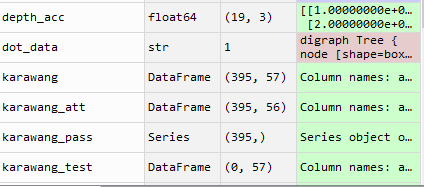
\includegraphics[width=4cm]{figures/1174009/tugas2/materi/hasil4.PNG}
		\caption{Hasil Soal 4.}
	\end{figure}

	\item Soal 5
	\hfill\break
	\lstinputlisting[firstline=57, lastline=60]{src/1174009/tugas2.py}
	Dari librari scikitlearn import modul tree. Kemudian definisikan variabel asahan dengan menggunakan DecisionClassifier. Kemudian pada variabel asahan terdapat Criterion yaitu suatu fungsi untuk mengukur kualitas split, setelah itu agar DecisionTreeClassifier dapat dijalankan gunakan perintah fit. Hasilnya adalah sebagai berikut :
	\begin{figure}[H]
	\centering
		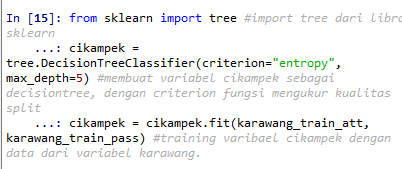
\includegraphics[width=4cm]{figures/1174009/tugas2/materi/hasil5.PNG}
		\caption{Hasil Soal 5.}
	\end{figure}

	\item Soal 6
	\hfill\break
	\lstinputlisting[firstline=65, lastline=71]{src/1174009/tugas2.py}
	Graphviz adalah perangkat lunak visualisasi grafik open source. Visualisasi grafik adalah cara mewakili informasi struktural sebagai diagram grafik dan jaringan abstrak. Hasilnya adalah sebagai berikut :
	\begin{figure}[H]
	\centering
		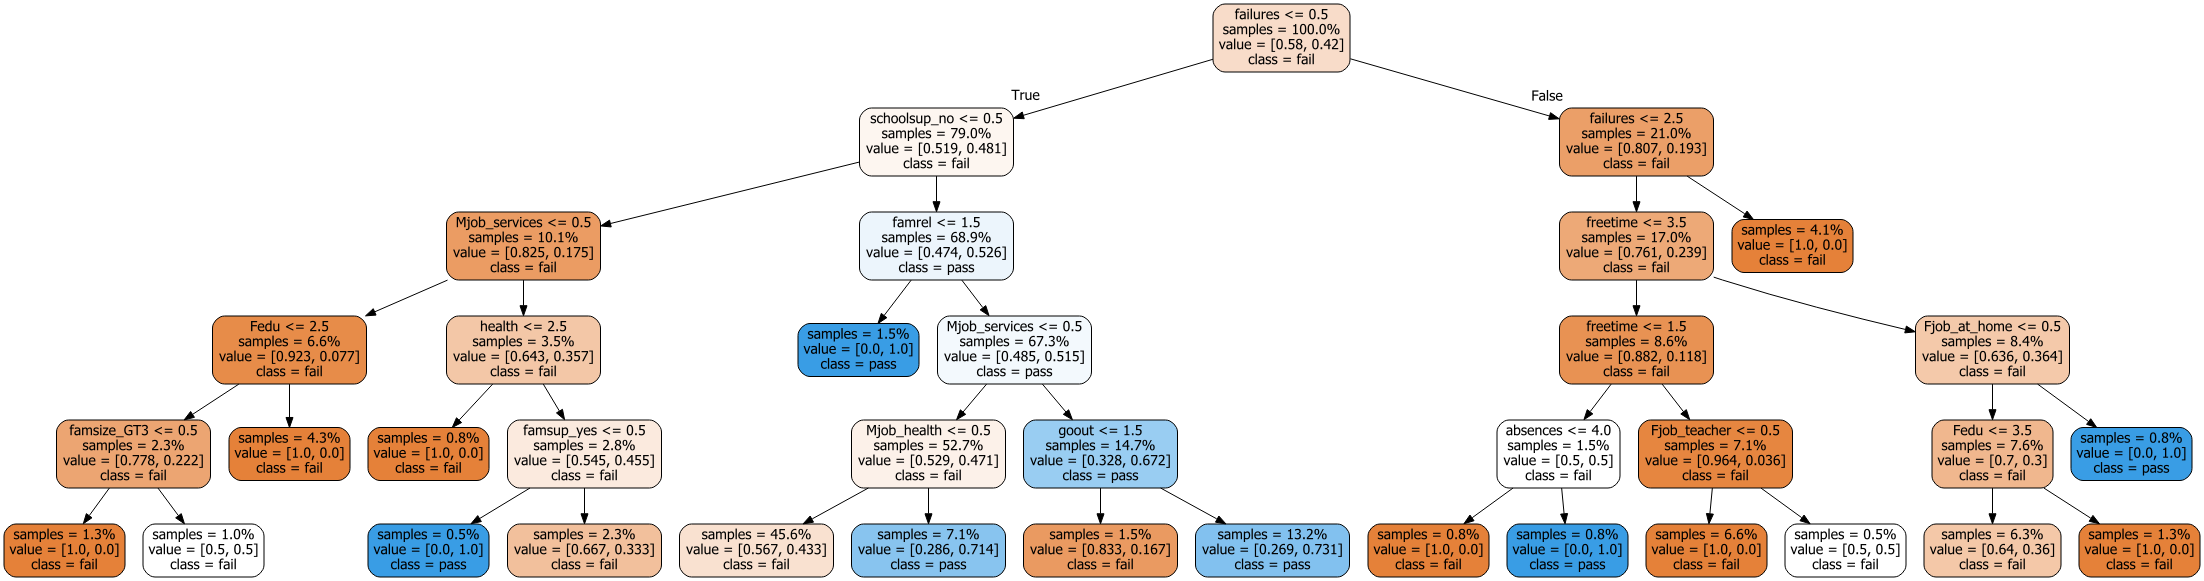
\includegraphics[width=4cm]{figures/1174009/tugas2/materi/hasil6.PNG}
		\caption{Hasil Soal 6.}
	\end{figure}

	\item Soal 7
	\hfill\break
	\lstinputlisting[firstline=76, lastline=79]{src/1174009/tugas2.py}
	Tree.export graphviz merupakan fungsi yang menghasilkan representasi Graphviz dari decision tree, yang kemudian ditulis ke outfile.Disini akan menyimpan classifiernya, akan meng ekspor file student performance jika salah akan mengembalikan nilai fail. Hasilnya adalah sebagai berikut :
	\begin{figure}[H]
	\centering
		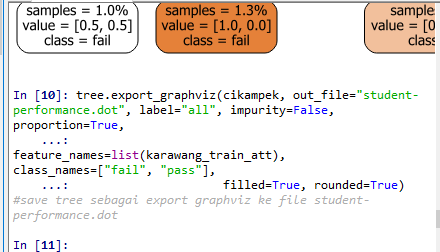
\includegraphics[width=4cm]{figures/1174009/tugas2/materi/hasil7.PNG}
		\caption{Hasil Soal 7.}
	\end{figure}

	\item Soal 8
	\hfill\break
	\lstinputlisting[firstline=84, lastline=86]{src/1174009/tugas2.py}
	Score juga disebut prediksi, dan merupakan proses menghasilkan nilai berdasarkan model pembelajaran mesin yang terlatih, diberi beberapa data input baru. Nilai atau skor yang dibuat dapat mewakili prediksi nilai masa depan, tetapi mereka juga mungkin mewakili kategori atau hasil yang mungkin. Jadi disini asahan akan memprediksi nilai dari medan test att dan test pass Hasilnya adalah sebagai berikut :
	\begin{figure}[H]
	\centering
		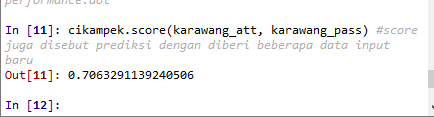
\includegraphics[width=4cm]{figures/1174009/tugas2/materi/hasil8.PNG}
		\caption{Hasil Soal 8.}
	\end{figure}

	\item Soal 9
	\hfill\break
	\lstinputlisting[firstline=91, lastline=94]{src/1174009/tugas2.py}
	Skrip ini akan mengevaluasi score dengan validasi silang. Dimana variabel scores berisikan crossvalscore yang merupakan fungsi pembantu pada estimator dan dataset. Kemudian akan menampilkan score rata rata dan kurang lebih dua standar deviasi yang mencakup 95 persen score. Hasilnya adalah sebagai berikut :
	\begin{figure}[H]
	\centering
		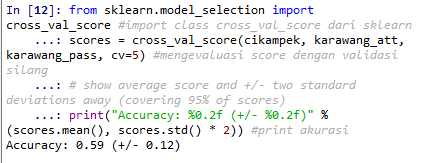
\includegraphics[width=4cm]{figures/1174009/tugas2/materi/hasil9.PNG}
		\caption{Hasil Soal 9.}
	\end{figure}

	\item Soal 10
	\hfill\break
	\lstinputlisting[firstline=99, lastline=104]{src/1174009/tugas2.py}
	Pada skrip ini menunjukkan seberapa dalam tree itu. Semakin dalam tree, semakin banyak perpecahan yang dimilikinya dan menangkap lebih banyak informasi tentang data. variabel asahan akan mendefinisikan tree nya yang kemudian variabel scores akan mengevaluasi score dengan validasi silang. disini mendefinisikan decision tree dengan kedalaman mulai dari 1 hingga 20. Hasilnya adalah sebagai berikut :
	\begin{figure}[H]
	\centering
		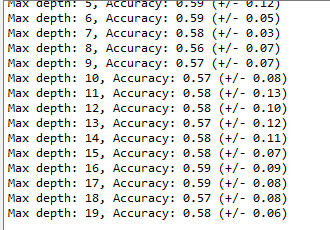
\includegraphics[width=4cm]{figures/1174009/tugas2/materi/hasil10.PNG}
		\caption{Hasil Soal 10.}
	\end{figure}

	\item Soal 11
	\hfill\break
	\lstinputlisting[firstline=109, lastline=119]{src/1174009/tugas2.py}
	Depth acc akan membuat array kosong dengan mengembalikan array baru dengan bentuk dan tipe yang diberikan, tanpa menginisialisasi entri. Dengan 19 sebagai bentuk array kosong, 3 sebagai output data-type dan float urutan kolomutama (gaya Fortran) dalam memori. variabel asahan yang akan melakukan split score akan mengvalidasi score secara silang. Hasilnya adalah sebagai berikut :
	\begin{figure}[H]
	\centering
		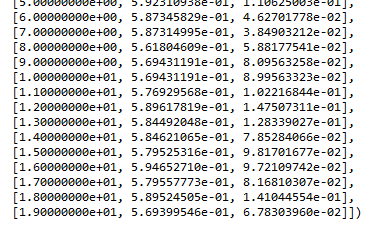
\includegraphics[width=4cm]{figures/1174009/tugas2/materi/hasil11.PNG}
		\caption{Hasil Soal 11.}
	\end{figure}

	\item Soal 12
	\hfill\break
	\lstinputlisting[firstline=124, lastline=127]{src/1174009/tugas2.py}
	Mengimpor librari dari matplotlib yaitu pylot sebagai plt fig dan ax menggunakan subplots untuk membuat gambar dan satu set subplot. axerrorbar akan membuat error bar kemudian grafik akan ditampilkan menggunakan show. Hasilnya adalah sebagai berikut :
	\begin{figure}[H]
	\centering
		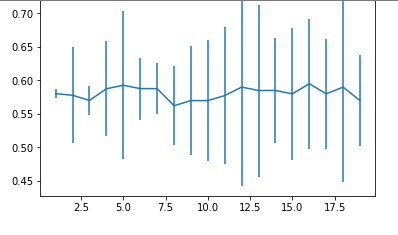
\includegraphics[width=4cm]{figures/1174009/tugas2/materi/hasil12.PNG}
		\caption{Hasil Soal 12.}
	\end{figure}
\end{enumerate}

\subsection{Penanganan Error}
\begin{enumerate}
	\item ScreenShoot Error
	\begin{figure}[H]
		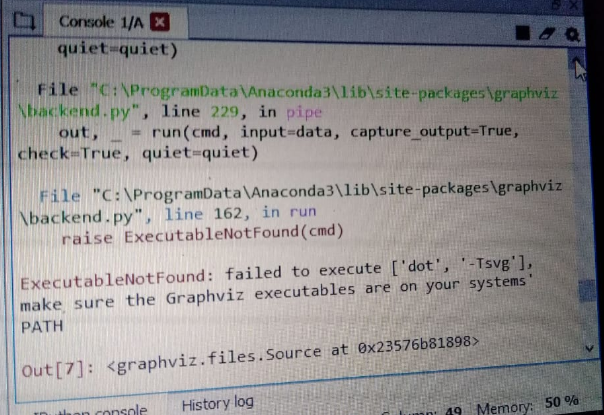
\includegraphics[width=4cm]{figures/1174009/tugas2/error/1.PNG}
		\centering
		\caption{ModuleNotFoundError}
	\end{figure}
	\begin{figure}[H]
		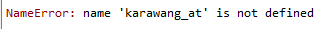
\includegraphics[width=4cm]{figures/1174009/tugas2/error/2.PNG}
		\centering
		\caption{NameError}
	\end{figure}
	\begin{figure}[H]
		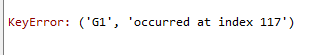
\includegraphics[width=4cm]{figures/1174009/tugas2/error/3.PNG}
		\centering
		\caption{KeyError}
	\end{figure}
	\item Tuliskan Kode Error dan Jenis Error
	\begin{itemize}
		\item ModuleNotFoundError
		\item NameError
		\item KeyError
	\end{itemize}
	\item Cara Penangan Error
	\begin{itemize}
		\item ModuleNotFoundError
		\hfill\break
		Error terdapat pada kesalahan modul graphviz yang belum di install, solusinya ialah menginstall library tersebut di anaconda.
		\item NameError
		\hfill\break
		Error terdapat pada penamaan alias pd yang tidak terdefenisikan, seharusnya jika variabel sate, maka sate juga.
		
		\item KeyError
		\hfill\break
		Key Error disebabkan oleh adanya kata kunci yang tidak terpanggil, disini adalah key (sate att), penanganannya yaitu disesuaikan kembali penamaannya saat proses train.
	\end{itemize}
\end{enumerate}
\subsection{Bukti Tidak Plagiat}
\begin{figure}[H]
\centering
	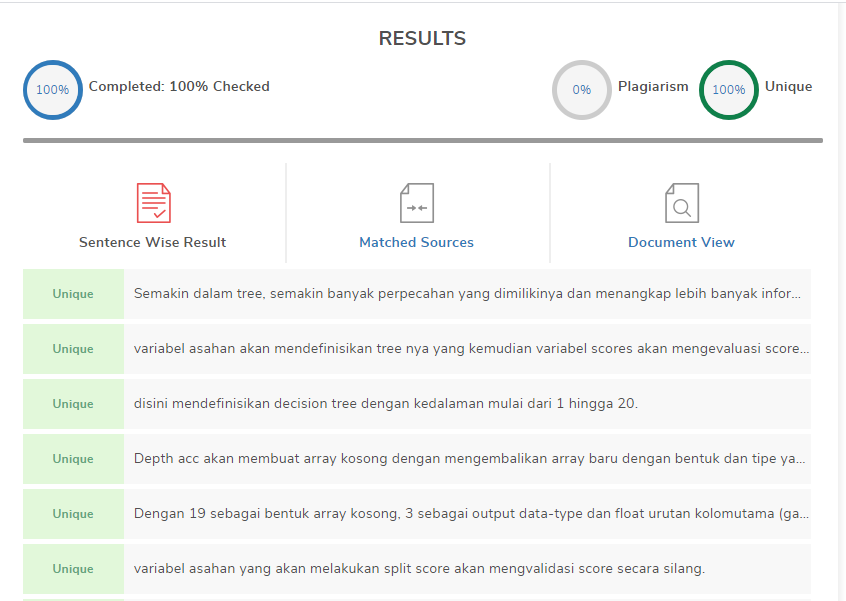
\includegraphics[width=4cm]{figures/1174009/tugas2/buktiplagiat/bukti.PNG}
	\caption{Bukti Tidak Melakukan Plagiat Chapter 2}
\end{figure}

